
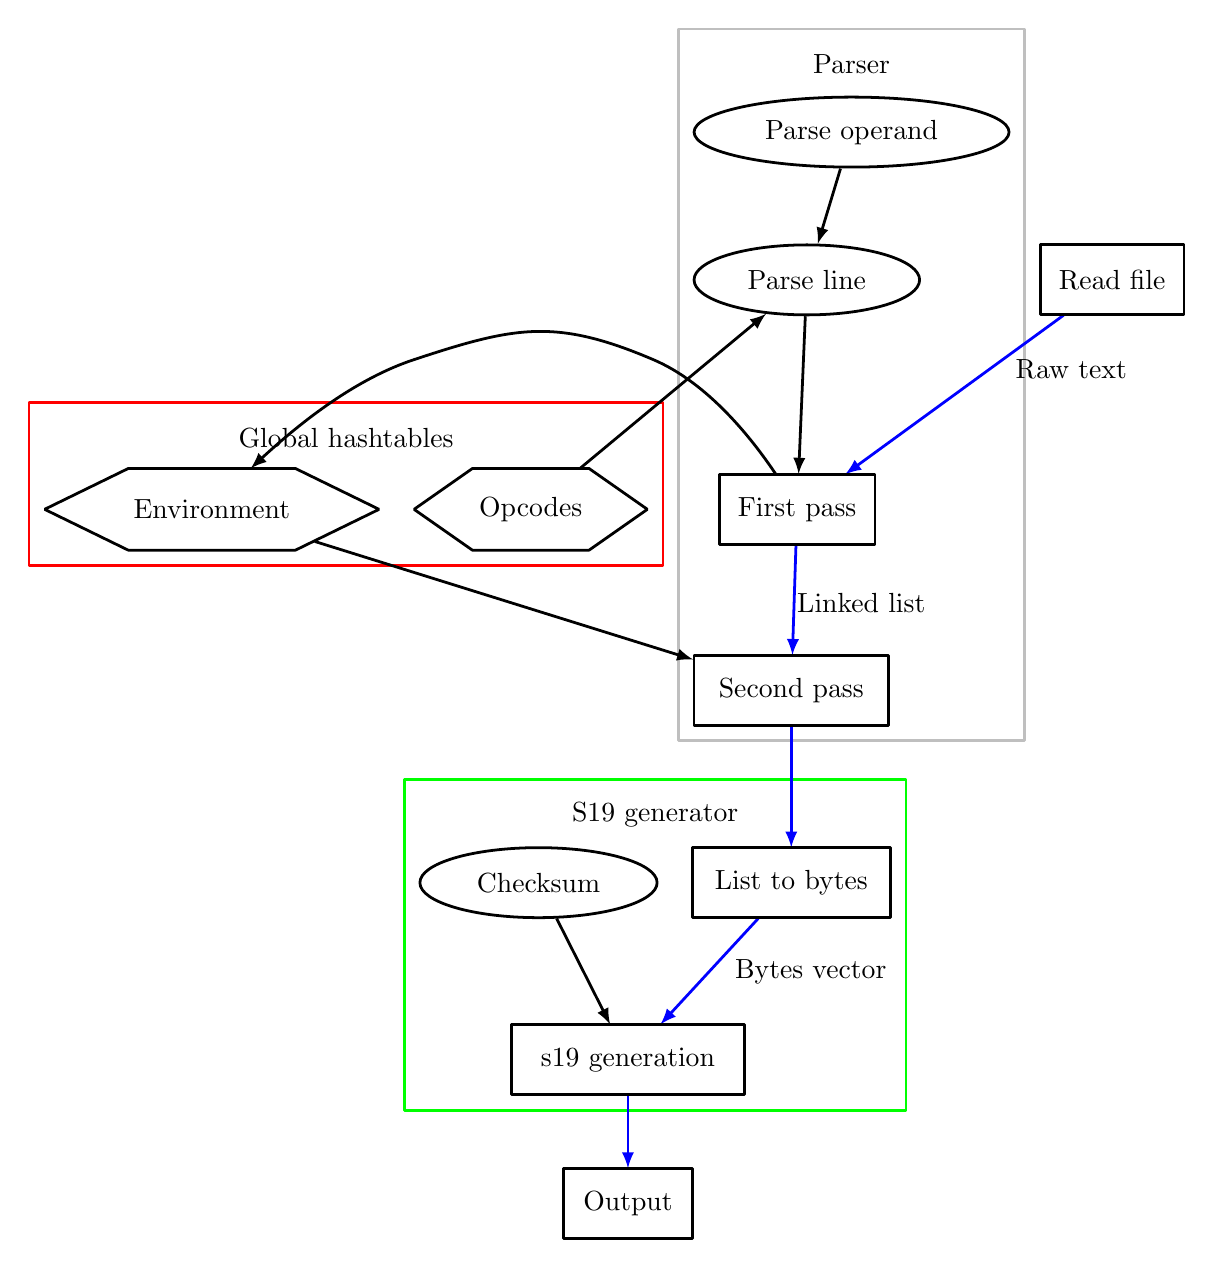
\begin{tikzpicture}[>=latex,line join=bevel,scale=0.7]
  \pgfsetlinewidth{1bp}
%%
\begin{scope}
  \pgfsetstrokecolor{black}
  \definecolor{strokecol}{rgb}{1.0,0.0,0.0};
  \pgfsetstrokecolor{strokecol}
  \draw (8bp,346bp) -- (8bp,430bp) -- (334bp,430bp) -- (334bp,346bp) -- cycle;
  \definecolor{strokecol}{rgb}{0.0,0.0,0.0};
  \pgfsetstrokecolor{strokecol}
  \draw (171bp,412bp) node {Global hashtables};
\end{scope}
\begin{scope}
  \pgfsetstrokecolor{black}
  \definecolor{strokecol}{rgb}{0.75,0.75,0.75};
  \pgfsetstrokecolor{strokecol}
  \draw (342bp,256bp) -- (342bp,622bp) -- (520bp,622bp) -- (520bp,256bp) -- cycle;
  \definecolor{strokecol}{rgb}{0.0,0.0,0.0};
  \pgfsetstrokecolor{strokecol}
  \draw (431bp,604bp) node {Parser};
\end{scope}
\begin{scope}
  \pgfsetstrokecolor{black}
  \definecolor{strokecol}{rgb}{0.0,1.0,0.0};
  \pgfsetstrokecolor{strokecol}
  \draw (201bp,66bp) -- (201bp,236bp) -- (459bp,236bp) -- (459bp,66bp) -- cycle;
  \definecolor{strokecol}{rgb}{0.0,0.0,0.0};
  \pgfsetstrokecolor{strokecol}
  \draw (330bp,218bp) node {S19 generator};
\end{scope}
  \pgfsetcolor{black}
  % Edge: file -> p1
  \pgfsetcolor{blue}
  \draw [->] (540.04bp,474.82bp) .. controls (512.13bp,454.49bp) and (466.82bp,421.48bp)  .. (427.72bp,393.01bp);
  \definecolor{strokecol}{rgb}{0.0,0.0,0.0};
  \pgfsetstrokecolor{strokecol}
  \draw (544bp,447bp) node {Raw text};
  % Edge: po -> pl
  \draw [->] (425.31bp,550.21bp) .. controls (422.67bp,541.47bp) and (419.47bp,530.89bp)  .. (413.62bp,511.57bp);
  % Edge: p1 -> env
  \draw [->] (392.04bp,393.07bp) .. controls (379.48bp,411.84bp) and (356.98bp,440.09bp)  .. (329bp,452bp) .. controls (278.7bp,473.42bp) and (257.91bp,469.13bp)  .. (206bp,452bp) .. controls (176.62bp,442.31bp) and (148.75bp,420.76bp)  .. (121.97bp,396.04bp);
  % Edge: ht -> pl
  \draw [->] (291.36bp,396.07bp) .. controls (316bp,416.55bp) and (353.35bp,447.59bp)  .. (387.05bp,475.59bp);
  % Edge: p1 -> p2
  \pgfsetcolor{blue}
  \draw [->] (402.41bp,356.63bp) .. controls (401.98bp,343.42bp) and (401.4bp,325.37bp)  .. (400.58bp,300.02bp);
  \definecolor{strokecol}{rgb}{0.0,0.0,0.0};
  \pgfsetstrokecolor{strokecol}
  \draw (436bp,327bp) node {Linked list};
  % Edge: chk -> s19
  \draw [->] (279.31bp,164.58bp) .. controls (285.9bp,151.55bp) and (294.85bp,133.85bp)  .. (306.86bp,110.08bp);
  % Edge: v -> s19
  \pgfsetcolor{blue}
  \draw [->] (383bp,164.58bp) .. controls (370.51bp,151.05bp) and (353.38bp,132.49bp)  .. (332.69bp,110.08bp);
  \definecolor{strokecol}{rgb}{0.0,0.0,0.0};
  \pgfsetstrokecolor{strokecol}
  \draw (410bp,137bp) node {Bytes vector};
  % Edge: pl -> p1
  \draw [->] (407.21bp,474.3bp) .. controls (406.4bp,455.2bp) and (405.13bp,425.31bp)  .. (403.77bp,393.22bp);
  % Edge: s19 -> output
  \pgfsetcolor{blue}
  \draw [->] (316bp,73.708bp) .. controls (316bp,65.464bp) and (316bp,55.538bp)  .. (316bp,36.082bp);
  % Edge: env -> p2
  \pgfsetcolor{black}
  \draw [->] (154.93bp,358.48bp) .. controls (206.73bp,342.31bp) and (285.54bp,317.72bp)  .. (349.55bp,297.75bp);
  % Edge: p2 -> v
  \pgfsetcolor{blue}
  \draw [->] (400bp,263.84bp) .. controls (400bp,249.19bp) and (400bp,228.31bp)  .. (400bp,201.04bp);
  % Node: p2
\begin{scope}
  \definecolor{strokecol}{rgb}{0.0,0.0,0.0};
  \pgfsetstrokecolor{strokecol}
  \draw (450bp,300bp) -- (350bp,300bp) -- (350bp,264bp) -- (450bp,264bp) -- cycle;
  \draw (400bp,282bp) node {Second pass};
\end{scope}
  % Node: s19
\begin{scope}
  \definecolor{strokecol}{rgb}{0.0,0.0,0.0};
  \pgfsetstrokecolor{strokecol}
  \draw (376bp,110bp) -- (256bp,110bp) -- (256bp,74bp) -- (376bp,74bp) -- cycle;
  \draw (316bp,92bp) node {s19 generation};
\end{scope}
  % Node: p1
\begin{scope}
  \definecolor{strokecol}{rgb}{0.0,0.0,0.0};
  \pgfsetstrokecolor{strokecol}
  \draw (443bp,393bp) -- (363bp,393bp) -- (363bp,357bp) -- (443bp,357bp) -- cycle;
  \draw (403bp,375bp) node {First pass};
\end{scope}
  % Node: file
\begin{scope}
  \definecolor{strokecol}{rgb}{0.0,0.0,0.0};
  \pgfsetstrokecolor{strokecol}
  \draw (602bp,511bp) -- (528bp,511bp) -- (528bp,475bp) -- (602bp,475bp) -- cycle;
  \draw (565bp,493bp) node {Read file};
\end{scope}
  % Node: chk
\begin{scope}
  \definecolor{strokecol}{rgb}{0.0,0.0,0.0};
  \pgfsetstrokecolor{strokecol}
  \draw (270bp,183bp) ellipse (61bp and 18bp);
  \draw (270bp,183bp) node {Checksum};
\end{scope}
  % Node: ht
\begin{scope}
  \definecolor{strokecol}{rgb}{0.0,0.0,0.0};
  \pgfsetstrokecolor{strokecol}
  \draw (326bp,375bp) -- (296bp,396bp) -- (236bp,396bp) -- (206bp,375bp) -- (236bp,354bp) -- (296bp,354bp) -- cycle;
  \draw (266bp,375bp) node {Opcodes};
\end{scope}
  % Node: env
\begin{scope}
  \definecolor{strokecol}{rgb}{0.0,0.0,0.0};
  \pgfsetstrokecolor{strokecol}
  \draw (188bp,375bp) -- (145bp,396bp) -- (59bp,396bp) -- (16bp,375bp) -- (59bp,354bp) -- (145bp,354bp) -- cycle;
  \draw (102bp,375bp) node {Environment};
\end{scope}
  % Node: v
\begin{scope}
  \definecolor{strokecol}{rgb}{0.0,0.0,0.0};
  \pgfsetstrokecolor{strokecol}
  \draw (451bp,201bp) -- (349bp,201bp) -- (349bp,165bp) -- (451bp,165bp) -- cycle;
  \draw (400bp,183bp) node {List to bytes};
\end{scope}
  % Node: output
\begin{scope}
  \definecolor{strokecol}{rgb}{0.0,0.0,0.0};
  \pgfsetstrokecolor{strokecol}
  \draw (349bp,36bp) -- (283bp,36bp) -- (283bp,0bp) -- (349bp,0bp) -- cycle;
  \draw (316bp,18bp) node {Output};
\end{scope}
  % Node: po
\begin{scope}
  \definecolor{strokecol}{rgb}{0.0,0.0,0.0};
  \pgfsetstrokecolor{strokecol}
  \draw (431bp,569bp) ellipse (81bp and 18bp);
  \draw (431bp,569bp) node {Parse operand};
\end{scope}
  % Node: pl
\begin{scope}
  \definecolor{strokecol}{rgb}{0.0,0.0,0.0};
  \pgfsetstrokecolor{strokecol}
  \draw (408bp,493bp) ellipse (58bp and 18bp);
  \draw (408bp,493bp) node {Parse line};
\end{scope}
%
\end{tikzpicture}

